% Drawing 154/02-5 -- folder 154, batch 02, archive page 25 (PDF page 26).
% Transcription: figures au bas de la page : un grand disque (bord vert) traversé par un arrangement de pseudo-droites orange, des régions coloriées en jaune, les points du bord numérotés $1$ à $12$ au crayon, de petits segments bleus marquant les extrémités ; à côté, un petit disque au bord vert et bleu, d'où partent vers l'intérieur dix « éventails » de traits orange et verts numérotés $1$ à $10$ --- le disque $\Delta'(D)$, vu au voisinage du bord
% Kind: pseudoline arrangement in a disk (Delta(D)); disk with fans near the boundary. Method 2 (schematic redraw from the facsimile). Status: partial.
% Notes: Foot of the page, right. A large disk with a green rim crossed by an orange arrangement drawn as a star: seven endpoints on the rim, each marked by a short blue stroke where two orange strands meet, narrow wedges at the rim coloured yellow; the rim points numbered 1 to 12 in pencil. Redrawn schematically: the seven endpoints and the pencil numbers are placed as on the page, but the strands are drawn as a regular {7/3} star joining them, which matches the look of the figure but not every crossing; the yellow wedges are left out. Beside it, a small disk with a green and blue rim from which ten fans of orange and green strokes point inwards, numbered 1 to 10 (the disk Delta'(D) seen near the boundary); the fans are placed evenly, which is approximate.
% Coordinates: 1 unit = 1 mm = 1/100 of the crop width (bbox in page fractions: [0.551, 0.335, 0.787, 0.525]).
% Redrawn by Claude (claude-opus-5-5), issue #73, 2026-11-07; not checked by a human; not compiled (no TeX in the session).
% Rights: reproduces part of the work -- behind RENDER_TRANSCRIPTS, never published by itself.
\documentclass[tikz,border=3pt]{standalone}
\usepackage{amsmath,amssymb}
\usetikzlibrary{patterns,arrows.meta}
\tikzset{Or/.style={orange!90!black}, Ye/.style={yellow!80!orange}, Lg/.style={green!60!black!70}, Dg/.style={green!45!black}, Br/.style={brown!80!black}, Rd/.style={red!85!black}, Bl/.style={blue!70!black}, Gy/.style={black!40}, pencil/.style={black!45}, struck/.style={black!35}, mark/.style={circle,draw,inner sep=1.3pt}, pt/.style={circle,fill,inner sep=0.9pt}, opt/.style={circle,draw,fill=white,inner sep=1.1pt}}
\begin{document}
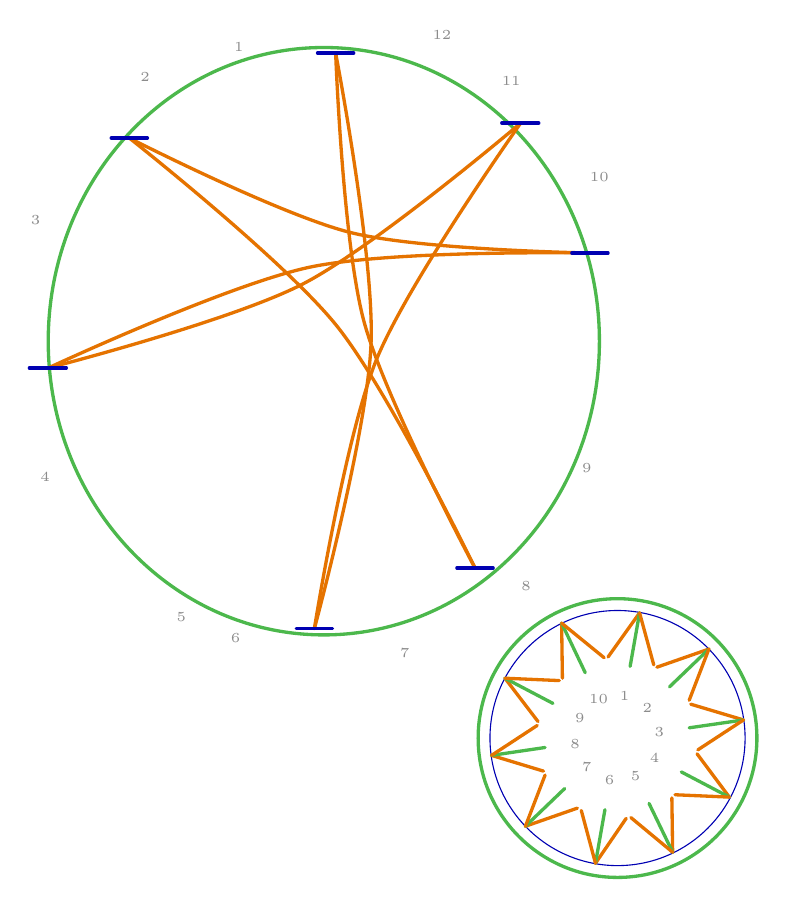
\begin{tikzpicture}[x=1mm,y=1mm,line cap=round,line join=round,font=\scriptsize]
\draw[Lg,very thick] (41.2,-43.1) ellipse[x radius=35, y radius=37.3];
\draw[Or,very thick] plot[smooth, tension=0.55] coordinates {(42.7,-6.5) (46.3,-40.6) (60.4,-71.9)};
\draw[Or,very thick] plot[smooth, tension=0.55] coordinates {(66.2,-15.4) (47.9,-45.4) (40,-79.6)};
\draw[Or,very thick] plot[smooth, tension=0.55] coordinates {(75,-31.9) (39.4,-33.7) (6.2,-46.5)};
\draw[Or,very thick] plot[smooth, tension=0.55] coordinates {(60.4,-71.9) (42.8,-41.1) (16.5,-17.3)};
\draw[Or,very thick] plot[smooth, tension=0.55] coordinates {(40,-79.6) (47.2,-43.3) (42.7,-6.5)};
\draw[Or,very thick] plot[smooth, tension=0.55] coordinates {(6.2,-46.5) (38.6,-35.8) (66.2,-15.4)};
\draw[Or,very thick] plot[smooth, tension=0.55] coordinates {(16.5,-17.3) (44.6,-29.3) (75,-31.9)};
\draw[Bl,very thick] (40.4,-6.5) -- (45,-6.5);
\draw[Bl,very thick] (63.8,-15.4) -- (68.5,-15.4);
\draw[Bl,very thick] (72.7,-31.9) -- (77.3,-31.9);
\draw[Bl,very thick] (58.1,-71.9) -- (62.7,-71.9);
\draw[Bl,very thick] (37.7,-79.6) -- (42.3,-79.6);
\draw[Bl,very thick] (3.8,-46.5) -- (8.5,-46.5);
\draw[Bl,very thick] (14.2,-17.3) -- (18.8,-17.3);
\node[inner sep=1pt,pencil] at (30.4,-5.8) {\tiny 1};
\node[inner sep=1pt,pencil] at (18.5,-9.6) {\tiny 2};
\node[inner sep=1pt,pencil] at (4.6,-27.7) {\tiny 3};
\node[inner sep=1pt,pencil] at (5.8,-60.4) {\tiny 4};
\node[inner sep=1pt,pencil] at (23.1,-78.1) {\tiny 5};
\node[inner sep=1pt,pencil] at (30,-80.8) {\tiny 6};
\node[inner sep=1pt,pencil] at (51.5,-82.7) {\tiny 7};
\node[inner sep=1pt,pencil] at (66.9,-74.2) {\tiny 8};
\node[inner sep=1pt,pencil] at (74.6,-59.2) {\tiny 9};
\node[inner sep=1pt,pencil] at (76.2,-22.3) {\tiny 10};
\node[inner sep=1pt,pencil] at (65,-10) {\tiny 11};
\node[inner sep=1pt,pencil] at (56.2,-4.2) {\tiny 12};
\draw[Lg,very thick] (78.5,-93.5) circle[radius=17.7];
\draw[Bl] (78.5,-93.5) circle[radius=16.2];
\draw[Or,very thick] (81.3,-77.6) -- (77.3,-83.2);
\draw[Lg,very thick] (81.3,-77.6) -- (80.1,-84.4);
\draw[Or,very thick] (81.3,-77.6) -- (83.1,-84.2);
\node[inner sep=1pt,pencil] at (79.4,-88.2) {\tiny 1};
\draw[Or,very thick] (90.1,-82.2) -- (83.5,-84.5);
\draw[Lg,very thick] (90.1,-82.2) -- (85.1,-87);
\draw[Or,very thick] (90.1,-82.2) -- (87.6,-88.7);
\node[inner sep=1pt,pencil] at (82.3,-89.7) {\tiny 2};
\draw[Or,very thick] (94.5,-91.2) -- (87.8,-89.2);
\draw[Lg,very thick] (94.5,-91.2) -- (87.6,-92.2);
\draw[Or,very thick] (94.5,-91.2) -- (88.7,-95);
\node[inner sep=1pt,pencil] at (83.8,-92.7) {\tiny 3};
\draw[Or,very thick] (92.7,-101) -- (88.6,-95.5);
\draw[Lg,very thick] (92.7,-101) -- (86.6,-97.8);
\draw[Or,very thick] (92.7,-101) -- (85.8,-100.7);
\node[inner sep=1pt,pencil] at (83.2,-96) {\tiny 4};
\draw[Or,very thick] (85.5,-108) -- (85.4,-101.1);
\draw[Lg,very thick] (85.5,-108) -- (82.5,-101.8);
\draw[Or,very thick] (85.5,-108) -- (80.2,-103.6);
\node[inner sep=1pt,pencil] at (80.8,-98.3) {\tiny 5};
\draw[Or,very thick] (75.7,-109.4) -- (79.6,-103.7);
\draw[Lg,very thick] (75.7,-109.4) -- (76.9,-102.6);
\draw[Or,very thick] (75.7,-109.4) -- (73.9,-102.7);
\node[inner sep=1pt,pencil] at (77.5,-98.8) {\tiny 6};
\draw[Or,very thick] (66.8,-104.7) -- (73.4,-102.4);
\draw[Lg,very thick] (66.8,-104.7) -- (71.8,-99.9);
\draw[Or,very thick] (66.8,-104.7) -- (69.3,-98.2);
\node[inner sep=1pt,pencil] at (74.6,-97.2) {\tiny 7};
\draw[Or,very thick] (62.5,-95.7) -- (69.1,-97.7);
\draw[Lg,very thick] (62.5,-95.7) -- (69.3,-94.7);
\draw[Or,very thick] (62.5,-95.7) -- (68.3,-91.9);
\node[inner sep=1pt,pencil] at (73.1,-94.2) {\tiny 8};
\draw[Or,very thick] (64.2,-85.9) -- (68.4,-91.4);
\draw[Lg,very thick] (64.2,-85.9) -- (70.3,-89.1);
\draw[Or,very thick] (64.2,-85.9) -- (71.1,-86.2);
\node[inner sep=1pt,pencil] at (73.7,-90.9) {\tiny 9};
\draw[Or,very thick] (71.4,-78.9) -- (71.5,-85.9);
\draw[Lg,very thick] (71.4,-78.9) -- (74.4,-85.2);
\draw[Or,very thick] (71.4,-78.9) -- (76.8,-83.3);
\node[inner sep=1pt,pencil] at (76.1,-88.6) {\tiny 10};
\end{tikzpicture}
\end{document}
